\subsubsection{Closed-form approach}

This section aims to explore alternative ways of calculating the steady state
probabilities using the connection between Markov chains and graph
theory.

\paragraph{Graph Theory}
In mathematics a graph \(G = (V, E)\) is a structure that consists of a set of
vertices \(V = \{v_1, v_2, \dots, v_n\}\) and a set of edges \(E = \{e_1, e_2,
\dots, e_m\}\) that connect the vertices together~\cite{bender2010lists}.
Every edge is expressed as \(e = (v_i, v_j)\) where \(v_i, v_j \in V\).

\begin{figure}[H]
    \centering
    \begin{tikzpicture}
    \node[state] (A) at (0,0) {A};
    \node[state] (B) at (0,3) {B};
    \node[state] (C) at (2.5,4) {C};
    \node[state] (D) at (2.5,1) {D};
    \node[state] (E) at (5,3) {E};

    \path (A) edge node {} (B);
    \path (B) edge node {} (C);
    \path (A) edge node {} (D);
    \path (D) edge node {} (C);
    \path (D) edge node {} (E);
    \path (C) edge node {} (E);
    \path (A) edge[bend right=60] node {} (E);
\end{tikzpicture}
    \caption{Example of a graph}
    \label{fig:example_of_graph}
\end{figure}

An additional type of graph is a directed graph, where the edges are directed
from one vertex to another.
In this case, the edges are expressed as \(e = (v_i, v_j)\) where \(v_i, v_j 
\in V\) and \((v_i, v_j) \neq (v_j, v_i)\)~\cite{balakrishnan2012textbook}.

\begin{figure}[H]
    \centering
    \begin{tikzpicture}
    \node[state] (A) at (0,0) {A};
    \node[state] (B) at (0,3) {B};
    \node[state] (C) at (2.5,4) {C};
    \node[state] (D) at (2.5,1) {D};
    \node[state] (E) at (5,3) {E};

    \draw[every loop]
        (A) edge node {} (B)
        (B) edge node {} (C)
        (A) edge node {} (D)
        (D) edge node {} (E)
        (D) edge node {} (C)
        (C) edge node {} (E)
        (E) edge[bend left=60] node {} (A)
    ;
\end{tikzpicture}
    \caption{Example of a graph}
    \label{fig:example_of_directed_graph}
\end{figure}

Furthermore, a weighted graph is a graph where each edge has a weight attached
to it~\cite{krukowski2021approximate}.
In this case, the edges are expressed as \(e = (v_i, v_j, w)\) where \(v_i, v_j
\in V\) and \(w \in \mathbb{R}\).

\begin{figure}[H]
    \centering
    \begin{tikzpicture}
    \node[state] (A) at (0,0) {A};
    \node[state] (B) at (0,3) {B};
    \node[state] (C) at (2.5,4) {C};
    \node[state] (D) at (2.5,1) {D};
    \node[state] (E) at (5,3) {E};

    \draw[every loop]
        (A) edge node[right] {4} (B)
        (B) edge node[above] {2} (C)
        (A) edge node[above] {3} (D)
        (D) edge node[above] {5} (E)
        (D) edge node[left] {7} (C)
        (C) edge node[above] {1} (E)
        (E) edge[bend left=60] node[above] {2} (A)
    ;
\end{tikzpicture}
    \caption{Example of a graph}
    \label{fig:example_of_weighted_directed_graph}
\end{figure}

\paragraph{A graph theoretic model underlying the Markov chain}
It can be assumed that a Markov chain model \(M\) can be translated as a
weighted directed graph \(G_M = (V, E)\) where \(V=S\) from
equation~(\ref{eq:definition_of_S_as_disjoint_union}) and \((v_i, v_j)\in E\) if
and only if \(q_{v_i, v_j}>0\), where \(v_i, v_j \in V\).
Furthermore, the weight of each edge is given by:

\[
    w(v_i, v_j) = q_{v_i, v_j}
\]

As described in Section~\ref{sec:queueing_section} the parameters considered as
inputs are:

\begin{itemize}
    \item the number of servers \(C\),
    \item the threshold \(T\),
    \item the capacity of node 1 \(N\),
    \item the capacity of node 2 \(M\).
\end{itemize}

These are the parameters that directly affect the structure of the Markov chain
as a graph.
Additional parameters of the model are the type 1 individuals arrival rate,
the type 2 individuals arrival rate and the service rate (\(\lambda_1,
\lambda_2, \mu\)).
More specifically, the way these parameters are translated into the model are:

\begin{itemize}
    \item \textbf{Number of servers (\(C\)):} Affects the weight of all edges
    \((v_i, v_j) \in E\) in the Markov chain that correspond to a service rate.
    These edges have a weight of:
    \begin{equation*}
        w_{(v_i, v_j)} = q_{v_i, v_j}
    \end{equation*}
    where \(q_{i,j}\) is defined in equation~(\ref{eq:markov_transition_rate}).
    Thus, the coefficients of the service rate have a lower bound of \(1\) and
    an upper bound of \(C\).
    \item \textbf{Threshold (\(T\)):} Determines the length of the left
    \textit{arm} of the model.
    In essence the threshold acts as a breakpoint between states where \(u=0\)
    and states where \(0 \leq u \leq M\).
    Increasing \(T\) results in having more set of states where \(u\) can only
    be \(0\).
    \item \textbf{Node 1 capacity (\(N\)):} Is the upper bound of \(v\)
    for all  states \((u,v)\).
    \item \textbf{Node 2 capacity (\(M\)):} Is the upper bound of \(u\)
    for all states \((u,v)\) such that \(v \geq T\).
\end{itemize}


\begin{figure}[H]
    \centering
    \scalebox{0.7}{
        \begin{tikzpicture}[-, node distance = 1cm, auto]
\node[state] (u0v0) {(0,0)};
\node[state, right=of u0v0] (u0v1) {(0,1)};
\draw[->](u0v0) edge[bend left] node {\( \Lambda \)} (u0v1);
\draw[->](u0v1) edge[bend left] node {\(\mu \)} (u0v0);
\node[state, right=of u0v1] (u0v2) {(0,2)};
\draw[->](u0v1) edge[bend left] node {\( \Lambda \)} (u0v2);
\draw[->](u0v2) edge[bend left] node {\(\mu \)} (u0v1);
\node[state, right=of u0v2] (u0v3) {(0,3)};
\draw[->](u0v2) edge[bend left] node {\( \Lambda \)} (u0v3);
\draw[->](u0v3) edge[bend left] node {\(\mu \)} (u0v2);
\node[state, below=of u0v3] (u1v3) {(1,3)};
\draw[->](u0v3) edge[bend left] node {\( \lambda_2 \)} (u1v3);
\draw[->](u1v3) edge[bend left] node {\(\mu \)} (u0v3);
\node[state, below=of u1v3] (u2v3) {(2,3)};
\draw[->](u1v3) edge[bend left] node {\( \lambda_2 \)} (u2v3);
\draw[->](u2v3) edge[bend left] node {\(\mu \)} (u1v3);
\node[state, right=of u0v3] (u0v4) {(0,4)};
\draw[->](u0v3) edge[bend left] node {\( \lambda_1 \)} (u0v4);
\draw[->](u0v4) edge[bend left] node {\(\mu \)} (u0v3);
\node[state, right=of u1v3] (u1v4) {(1,4)};
\draw[->](u1v3) edge[bend left] node {\( \lambda_1 \)} (u1v4);
\draw[->](u1v4) edge[bend left] node {\(\mu \)} (u1v3);
\draw[->](u0v4) edge node {\( \lambda_2 \)} (u1v4);
\node[state, right=of u2v3] (u2v4) {(2,4)};
\draw[->](u2v3) edge[bend left] node {\( \lambda_1 \)} (u2v4);
\draw[->](u2v4) edge[bend left] node {\(\mu \)} (u2v3);
\draw[->](u1v4) edge node {\( \lambda_2 \)} (u2v4);
\node[state, right=of u0v4] (u0v5) {(0,5)};
\draw[->](u0v4) edge[bend left] node {\( \lambda_1 \)} (u0v5);
\draw[->](u0v5) edge[bend left] node {\(\mu \)} (u0v4);
\node[state, right=of u1v4] (u1v5) {(1,5)};
\draw[->](u1v4) edge[bend left] node {\( \lambda_1 \)} (u1v5);
\draw[->](u1v5) edge[bend left] node {\(\mu \)} (u1v4);
\draw[->](u0v5) edge node {\( \lambda_2 \)} (u1v5);
\node[state, right=of u2v4] (u2v5) {(2,5)};
\draw[->](u2v4) edge[bend left] node {\( \lambda_1 \)} (u2v5);
\draw[->](u2v5) edge[bend left] node {\(\mu \)} (u2v4);
\draw[->](u1v5) edge node {\( \lambda_2 \)} (u2v5);
\end{tikzpicture}
        }
    \caption{\(C=1, T=3, N=5, M=2\)}
    \label{fig:Markov_1352_example_for_closed_form}
\end{figure}

In Figure~\ref{fig:Markov_1352_example_for_closed_form} an example of such a
Markov model is shown where \(C=1\), \(T=3\) which means that the \textit{left
arm} of the model has a length of \(3\), \(N=5\) that indicates that the
right-most states \((u,v)\) are of the form \((u,5)\) and \(M=2\) that
equivalently shows that the bottom states are of the form \((2,v)\).

\paragraph{Spanning trees}

A \textit{spanning tree} is defined as a subset of the graph that visits all
the vertices of the graph and does not include any
cycles~\cite{bollobas1998modern}.
Unlike undirected spanning trees, directed ones also have a root which means
that a \textit{directed spanning tree} that is rooted at a vertex \(v\) has to
have a path from any other vertex to vertex \(v\)~\cite{levine2011sandpile}.
For example, consider the graph shown in Figure~\ref{fig:example_spanning_tree}.
The graph points out a spanning tree that is rooted at vertex 3.


\begin{figure}[H]
    \centering
    \begin{tikzpicture}
        \node[state](u1){1};
        \node[state, right=of u1](u2){2};
        \node[state, right=of u2](u3){3};
        \node[state, right=of u3](u4){4};
        \node[state, below=of u2](u5){5};
        \node[state, below=of u3](u6){6};
        \node[state, below=of u4](u7){7};
        \draw[->, thick] (u1) -- (u2);
        \draw[->, thick] (u2) -- (u3);
        \draw[->, thick] (u4) -- (u3);
        \draw[->, thick] (u5) -- (u2);
        \draw[->, thick] (u6) -- (u5);
        \draw[->, thick] (u7) -- (u6);
    \end{tikzpicture}
    \caption{Spanning tree of a graph rooted at vertex 3}
    \label{fig:example_spanning_tree}
\end{figure}

Let us denote the set of all spanning trees of a graph \(G\) as \(T(G)\)
and the subset of \(T(G)\) that includes only the spanning trees that are rooted
at vertex \(v\) as \(T_v(G)\).
The weight of a spanning tree \(t\) can be defined as the product of the weights
of the edges it contains~\cite{williams2022combinatorics}:

\[
    w(t)=\prod_{e \in t} w(e)
\]


\textbf{Theorem: Markov chain tree theorem}~\cite{broder1989generating}:\newline
\textit{Let M be an irreducible Markov chain on n states with stationary
distribution \(\pi_1, \pi_2, \dots, \pi_n\).
Let \(G_M\) be the directed graph associated with \(M\).
Then the probability of being at state \(u\) is given by:}

\begin{equation}\label{markov-chain-tree-theorem}
    \pi_i = \frac{\sum_{t \in T_i(G_M)} w(t)}{\sum_{t \in T(G_M)}w(t)}
\end{equation}

Equation~\ref{markov-chain-tree-theorem} states that the probability of being at
state \(u\) can be found by dividing the sum of the weights of all trees in
\(T_u(G)\) by the sum of the weights of all tress in \(T(G)\).
Let us ignore the denominator of that fraction for now and focus only on the
numerator denoted as \(\tilde{\pi}_i=\sum_{t \in T_i(G_M)} w(t)\).
Another useful theorem that can be utilised is Kirchhoff's theorem that gives
some useful insights on the number of spanning trees of a graph.

\textbf{Theorem: Kirchhoff's theorem}~\cite{chaiken1978matrix}:\newline
\textit{The number of directed spanning trees rooted at a state \(i\) can be
found by calculating the determinant of the Laplacian matrix \(Q\) of the
directed graph and removing row \(i\) and column \(i\).}


\paragraph{Spanning Trees rooted at \((0,0)\)}

Let us now consider some examples of spanning trees that are rooted at
\((0,0)\).
For each of the following examples the complete graph \(G\) is shown, then all
possible trees of \(T_{(0,0)}(G)\) along with the weight associated with each
spanning tree.
As well as this, the sum of all the weights of the spanning trees denoted by
\(\tilde{\pi}_{(0,0)}\) is also included.


\begin{figure}[H]
    \centering
    \begin{tikzpicture}[-, node distance = 0.8cm, auto]
\node[state] (u0v0) {(0,0)};
\node[state, right=of u0v0] (u0v1) {(0,1)};
\draw[->](u0v0) edge[bend left] node {\( \Lambda \)} (u0v1);
\draw[->](u0v1) edge[bend left] node {\(\mu \)} (u0v0);
\node[state, below=of u0v1] (u1v1) {(1,1)};
\draw[->](u0v1) edge[bend left] node {\( \lambda_2 \)} (u1v1);
\draw[->](u1v1) edge[bend left] node {\(\mu \)} (u0v1);
\node[state, right=of u0v1] (u0v2) {(0,2)};
\draw[->](u0v1) edge[bend left] node {\( \lambda_1 \)} (u0v2);
\draw[->](u0v2) edge[bend left] node {\(\mu \)} (u0v1);
\node[state, right=of u1v1] (u1v2) {(1,2)};
\draw[->](u1v1) edge[bend left] node {\( \lambda_1 \)} (u1v2);
\draw[->](u1v2) edge[bend left] node {\(\mu \)} (u1v1);
\draw[->](u0v2) edge node {\( \lambda_2 \)} (u1v2);
\end{tikzpicture}
\end{figure}

\begin{multicols}{2}
    \begin{center}
        

\begin{tikzpicture}[-, node distance = 1cm, auto]
\node[state] (u0v0) {(0,0)};
\node[state, right=of u0v0] (u0v1) {(0,1)};
\draw[->](u0v1) edge node {\(\mu \)} (u0v0);
\node[state, below=of u0v1] (u1v1) {(1,1)};
\draw[->](u1v1) edge node {\(\mu \)} (u0v1);
\node[state, right=of u0v1] (u0v2) {(0,2)};
\node[state, right=of u1v1] (u1v2) {(1,2)};
\draw[->](u1v2) edge node {\(\mu \)} (u1v1);
\draw[->](u0v2) edge node {\(\lambda_2 \)} (u1v2);
\end{tikzpicture}
    \end{center}

    \begin{flalign*}
        \xrightarrow{\hspace*{2cm}} \hspace{1cm} \lambda_2 \mu^3
    \end{flalign*}
\end{multicols}


\begin{multicols}{2}
    \begin{center}
        

\begin{tikzpicture}[-, node distance = 1cm, auto]
\node[state] (u0v0) {(0,0)};
\node[state, right=of u0v0] (u0v1) {(0,1)};
\draw[->](u0v1) edge node {\(\mu \)} (u0v0);
\node[state, below=of u0v1] (u1v1) {(1,1)};
\draw[->](u1v1) edge node {\(\mu \)} (u0v1);
\node[state, right=of u0v1] (u0v2) {(0,2)};
\node[state, right=of u1v1] (u1v2) {(1,2)};
\draw[->](u1v2) edge node {\(\mu \)} (u1v1);
\draw[->](u0v2) edge node {\(\mu \)} (u0v1);
\end{tikzpicture}
    \end{center}

    \begin{flalign*}
        \xrightarrow{\hspace*{2cm}} \hspace{1cm} \mu^4
    \end{flalign*}
\end{multicols}

\begin{equation*}
    \tilde{\pi}_{(0,0)} = \mu^4 + \lambda_2 \mu^3
\end{equation*}


\begin{figure}[H]
    \centering
    \begin{tikzpicture}[-, node distance = 1cm, auto]
\node[state] (u0v0) {(0,0)};
\node[state, right=of u0v0] (u0v1) {(0,1)};
\draw[->](u0v0) edge[bend left] node {\( \Lambda \)} (u0v1);
\draw[->](u0v1) edge[bend left] node {\(\mu \)} (u0v0);
\node[state, below=of u0v1] (u1v1) {(1,1)};
\draw[->](u0v1) edge[bend left] node {\( \lambda_2 \)} (u1v1);
\draw[->](u1v1) edge[bend left] node {\(\mu \)} (u0v1);
\node[state, right=of u0v1] (u0v2) {(0,2)};
\draw[->](u0v1) edge[bend left] node {\( \lambda_1 \)} (u0v2);
\draw[->](u0v2) edge[bend left] node {\(\mu \)} (u0v1);
\node[state, right=of u1v1] (u1v2) {(1,2)};
\draw[->](u1v1) edge[bend left] node {\( \lambda_1 \)} (u1v2);
\draw[->](u1v2) edge[bend left] node {\(\mu \)} (u1v1);
\draw[->](u0v2) edge node {\( \lambda_2 \)} (u1v2);
\node[state, right=of u0v2] (u0v3) {(0,3)};
\draw[->](u0v2) edge[bend left] node {\( \lambda_1 \)} (u0v3);
\draw[->](u0v3) edge[bend left] node {\(\mu \)} (u0v2);
\node[state, right=of u1v2] (u1v3) {(1,3)};
\draw[->](u1v2) edge[bend left] node {\( \lambda_1 \)} (u1v3);
\draw[->](u1v3) edge[bend left] node {\(\mu \)} (u1v2);
\draw[->](u0v3) edge node {\( \lambda_2 \)} (u1v3);
\end{tikzpicture}
\end{figure}


\begin{multicols}{2}
    \begin{figure}[H]
        \centering
        \scalebox{0.7}{
            

\begin{tikzpicture}[-, node distance = 1cm, auto]
\node[state] (u0v0) {(0,0)};
\node[state, right=of u0v0] (u0v1) {(0,1)};
\draw[->](u0v1) edge node {\(\mu \)} (u0v0);
\node[state, below=of u0v1] (u1v1) {(1,1)};
\draw[->](u1v1) edge node {\(\mu \)} (u0v1);
\node[state, right=of u0v1] (u0v2) {(0,2)};
\node[state, right=of u1v1] (u1v2) {(1,2)};
\draw[->](u1v2) edge node {\(\mu \)} (u1v1);
\node[state, right=of u0v2] (u0v3) {(0,3)};
\node[state, right=of u1v2] (u1v3) {(1,3)};
\draw[->](u1v3) edge node {\(\mu \)} (u1v2);
\draw[->](u0v2) edge node {\(\lambda_2 \)} (u1v2);
\draw[->](u0v3) edge node {\(\lambda_2 \)} (u1v3);
\end{tikzpicture}}
    \end{figure}

    \begin{flalign*}
        \xrightarrow{\hspace*{2cm}} \hspace{1cm} (\lambda_2)^2 \mu^4
    \end{flalign*}
\end{multicols}

\begin{multicols}{2}
    \begin{figure}[H]
        \centering
        \scalebox{0.7}{
            

\begin{tikzpicture}[-, node distance = 1cm, auto]
\node[state] (u0v0) {(0,0)};
\node[state, right=of u0v0] (u0v1) {(0,1)};
\draw[->](u0v1) edge node {\(\mu \)} (u0v0);
\node[state, below=of u0v1] (u1v1) {(1,1)};
\draw[->](u1v1) edge node {\(\mu \)} (u0v1);
\node[state, right=of u0v1] (u0v2) {(0,2)};
\node[state, right=of u1v1] (u1v2) {(1,2)};
\draw[->](u1v2) edge node {\(\mu \)} (u1v1);
\node[state, right=of u0v2] (u0v3) {(0,3)};
\node[state, right=of u1v2] (u1v3) {(1,3)};
\draw[->](u1v3) edge node {\(\mu \)} (u1v2);
\draw[->](u0v2) edge node {\(\mu \)} (u0v1);
\draw[->](u0v3) edge node {\(\lambda_2 \)} (u1v3);
\end{tikzpicture}}
    \end{figure}

    \begin{flalign*}
        \xrightarrow{\hspace*{2cm}} \hspace{1cm} \lambda_2 \mu^5
    \end{flalign*}
\end{multicols}

\begin{multicols}{2}
    \begin{figure}[H]
        \centering
        \scalebox{0.7}{
            

\begin{tikzpicture}[-, node distance = 1cm, auto]
\node[state] (u0v0) {(0,0)};
\node[state, right=of u0v0] (u0v1) {(0,1)};
\draw[->](u0v1) edge node {\(\mu \)} (u0v0);
\node[state, below=of u0v1] (u1v1) {(1,1)};
\draw[->](u1v1) edge node {\(\mu \)} (u0v1);
\node[state, right=of u0v1] (u0v2) {(0,2)};
\node[state, right=of u1v1] (u1v2) {(1,2)};
\draw[->](u1v2) edge node {\(\mu \)} (u1v1);
\node[state, right=of u0v2] (u0v3) {(0,3)};
\node[state, right=of u1v2] (u1v3) {(1,3)};
\draw[->](u1v3) edge node {\(\mu \)} (u1v2);
\draw[->](u0v2) edge node {\(\lambda_2 \)} (u1v2);
\draw[->](u0v3) edge node {\(\mu \)} (u0v2);
\end{tikzpicture}}
    \end{figure}

    \begin{flalign*}
        \xrightarrow{\hspace*{2cm}} \hspace{1cm} \lambda_2 \mu^5
    \end{flalign*}
\end{multicols}

\begin{multicols}{2}
    \begin{figure}[H]
        \centering
        \scalebox{0.7}{
            

\begin{tikzpicture}[-, node distance = 1cm, auto]
\node[state] (u0v0) {(0,0)};
\node[state, right=of u0v0] (u0v1) {(0,1)};
\draw[->](u0v1) edge node {\(\mu \)} (u0v0);
\node[state, below=of u0v1] (u1v1) {(1,1)};
\draw[->](u1v1) edge node {\(\mu \)} (u0v1);
\node[state, right=of u0v1] (u0v2) {(0,2)};
\node[state, right=of u1v1] (u1v2) {(1,2)};
\draw[->](u1v2) edge node {\(\mu \)} (u1v1);
\node[state, right=of u0v2] (u0v3) {(0,3)};
\node[state, right=of u1v2] (u1v3) {(1,3)};
\draw[->](u1v3) edge node {\(\mu \)} (u1v2);
\draw[->](u0v2) edge node {\(\lambda_1 \)} (u0v3);
\draw[->](u0v3) edge node {\(\lambda_2 \)} (u1v3);
\end{tikzpicture}}
    \end{figure}

    \begin{flalign*}
        \xrightarrow{\hspace*{2cm}} \hspace{1cm} \lambda_2 \lambda_1 \mu^4
    \end{flalign*}
\end{multicols}

\begin{multicols}{2}
    \begin{figure}[H]
        \centering
        \scalebox{0.7}{
            

\begin{tikzpicture}[-, node distance = 1cm, auto]
\node[state] (u0v0) {(0,0)};
\node[state, right=of u0v0] (u0v1) {(0,1)};
\draw[->](u0v1) edge node {\(\mu \)} (u0v0);
\node[state, below=of u0v1] (u1v1) {(1,1)};
\draw[->](u1v1) edge node {\(\mu \)} (u0v1);
\node[state, right=of u0v1] (u0v2) {(0,2)};
\node[state, right=of u1v1] (u1v2) {(1,2)};
\draw[->](u1v2) edge node {\(\mu \)} (u1v1);
\node[state, right=of u0v2] (u0v3) {(0,3)};
\node[state, right=of u1v2] (u1v3) {(1,3)};
\draw[->](u1v3) edge node {\(\mu \)} (u1v2);
\draw[->](u0v2) edge node {\(\mu \)} (u0v1);
\draw[->](u0v3) edge node {\(\mu \)} (u0v2);
\end{tikzpicture}}
    \end{figure}

    \begin{flalign*}
        \xrightarrow{\hspace*{2cm}} \hspace{1cm} \mu^6
    \end{flalign*}
\end{multicols}

\begin{equation*}
    \tilde{\pi}_{(0,0)} = (\lambda_2)^2 \mu^4 + 2 \lambda_2 \mu^5 +
    \lambda_2 \lambda_1 \mu^4 + \mu^6
\end{equation*}


\begin{figure}[H]
    \centering
    \begin{tikzpicture}[-, node distance = 1cm, auto]
\node[state] (u0v0) {(0,0)};
\node[state, right=of u0v0] (u0v1) {(0,1)};
\draw[->](u0v0) edge[bend left] node {\( \Lambda \)} (u0v1);
\draw[->](u0v1) edge[bend left] node {\(\mu \)} (u0v0);
\node[state, below=of u0v1] (u1v1) {(1,1)};
\draw[->](u0v1) edge[bend left] node {\( \lambda_2 \)} (u1v1);
\draw[->](u1v1) edge[bend left] node {\(\mu \)} (u0v1);
\node[state, below=of u1v1] (u2v1) {(2,1)};
\draw[->](u1v1) edge[bend left] node {\( \lambda_2 \)} (u2v1);
\draw[->](u2v1) edge[bend left] node {\(\mu \)} (u1v1);
\node[state, right=of u0v1] (u0v2) {(0,2)};
\draw[->](u0v1) edge[bend left] node {\( \lambda_1 \)} (u0v2);
\draw[->](u0v2) edge[bend left] node {\(\mu \)} (u0v1);
\node[state, right=of u1v1] (u1v2) {(1,2)};
\draw[->](u1v1) edge[bend left] node {\( \lambda_1 \)} (u1v2);
\draw[->](u1v2) edge[bend left] node {\(\mu \)} (u1v1);
\draw[->](u0v2) edge node {\( \lambda_2 \)} (u1v2);
\node[state, right=of u2v1] (u2v2) {(2,2)};
\draw[->](u2v1) edge[bend left] node {\( \lambda_1 \)} (u2v2);
\draw[->](u2v2) edge[bend left] node {\(\mu \)} (u2v1);
\draw[->](u1v2) edge node {\( \lambda_2 \)} (u2v2);
\end{tikzpicture}
\end{figure}

\begin{multicols}{4}
    \begin{figure}[H]
        \centering
        \scalebox{0.48}{
            

\begin{tikzpicture}[-, node distance = 1cm, auto]
\node[state] (u0v0) {(0,0)};
\node[state, right=of u0v0] (u0v1) {(0,1)};
\draw[->](u0v1) edge node {\(\mu \)} (u0v0);
\node[state, below=of u0v1] (u1v1) {(1,1)};
\draw[->](u1v1) edge node {\(\mu \)} (u0v1);
\node[state, below=of u1v1] (u2v1) {(2,1)};
\draw[->](u2v1) edge node {\(\mu \)} (u1v1);
\node[state, right=of u0v1] (u0v2) {(0,2)};
\node[state, right=of u1v1] (u1v2) {(1,2)};
\node[state, right=of u2v1] (u2v2) {(2,2)};
\draw[->](u2v2) edge node {\(\mu \)} (u2v1);
\draw[->](u0v2) edge node {\(\lambda_2 \)} (u1v2);
\draw[->](u1v2) edge node {\(\lambda_2 \)} (u2v2);
\end{tikzpicture}}
    \end{figure}
    \vspace*{\fill}
    \columnbreak
    \vspace*{0cm}
    \begin{equation*}
        (\lambda_2)^2 \mu^4
    \end{equation*}
    \vspace*{\fill}
    \columnbreak
    \begin{figure}[H]
        \centering
        \scalebox{0.48}{
            

\begin{tikzpicture}[-, node distance = 1cm, auto]
\node[state] (u0v0) {(0,0)};
\node[state, right=of u0v0] (u0v1) {(0,1)};
\draw[->](u0v1) edge node {\(\mu \)} (u0v0);
\node[state, below=of u0v1] (u1v1) {(1,1)};
\draw[->](u1v1) edge node {\(\mu \)} (u0v1);
\node[state, below=of u1v1] (u2v1) {(2,1)};
\draw[->](u2v1) edge node {\(\mu \)} (u1v1);
\node[state, right=of u0v1] (u0v2) {(0,2)};
\node[state, right=of u1v1] (u1v2) {(1,2)};
\node[state, right=of u2v1] (u2v2) {(2,2)};
\draw[->](u2v2) edge node {\(\mu \)} (u2v1);
\draw[->](u0v2) edge node {\(\mu \)} (u0v1);
\draw[->](u1v2) edge node {\(\lambda_2 \)} (u2v2);
\end{tikzpicture}}
    \end{figure}
    \vspace*{\fill}
    \columnbreak
    \vspace*{0.3cm}
    \begin{equation*}
        \lambda_2 \mu^5
    \end{equation*}
\end{multicols}

\newpage

\begin{multicols}{4}
    \begin{figure}[H]
        \centering
        \scalebox{0.48}{
            

\begin{tikzpicture}[-, node distance = 1cm, auto]
\node[state] (u0v0) {(0,0)};
\node[state, right=of u0v0] (u0v1) {(0,1)};
\draw[->](u0v1) edge node {\(\mu \)} (u0v0);
\node[state, below=of u0v1] (u1v1) {(1,1)};
\draw[->](u1v1) edge node {\(\mu \)} (u0v1);
\node[state, below=of u1v1] (u2v1) {(2,1)};
\draw[->](u2v1) edge node {\(\mu \)} (u1v1);
\node[state, right=of u0v1] (u0v2) {(0,2)};
\node[state, right=of u1v1] (u1v2) {(1,2)};
\node[state, right=of u2v1] (u2v2) {(2,2)};
\draw[->](u2v2) edge node {\(\mu \)} (u2v1);
\draw[->](u0v2) edge node {\(\lambda_2 \)} (u1v2);
\draw[->](u1v2) edge node {\(\mu \)} (u1v1);
\end{tikzpicture}}
    \end{figure}
    \vspace*{\fill}
    \columnbreak
    % \vspace*{0.3cm}
    \begin{equation*}
        \lambda_2 \mu^5
    \end{equation*}
    \vspace*{\fill}
    \columnbreak
    \begin{figure}[H]
        \centering
        \scalebox{0.48}{
            

\begin{tikzpicture}[-, node distance = 1cm, auto]
\node[state] (u0v0) {(0,0)};
\node[state, right=of u0v0] (u0v1) {(0,1)};
\draw[->](u0v1) edge node {\(\mu \)} (u0v0);
\node[state, below=of u0v1] (u1v1) {(1,1)};
\draw[->](u1v1) edge node {\(\mu \)} (u0v1);
\node[state, below=of u1v1] (u2v1) {(2,1)};
\draw[->](u2v1) edge node {\(\mu \)} (u1v1);
\node[state, right=of u0v1] (u0v2) {(0,2)};
\node[state, right=of u1v1] (u1v2) {(1,2)};
\node[state, right=of u2v1] (u2v2) {(2,2)};
\draw[->](u2v2) edge node {\(\mu \)} (u2v1);
\draw[->](u0v2) edge node {\(\mu \)} (u0v1);
\draw[->](u1v2) edge node {\(\mu \)} (u1v1);
\end{tikzpicture}}
    \end{figure}
    \vspace*{\fill}
    \columnbreak
    % \vspace*{0.3cm}
    \begin{equation*}
        \mu^6
    \end{equation*}
\end{multicols}


\begin{equation*}
    \tilde{\pi}_{(0,0)} = (\lambda_2)^2 \mu^4 + 2 \lambda_2 \mu^5 + \mu^6
\end{equation*}

\paragraph{Conjecture of adding rows}

Let us consider three Markov models with the same number of servers \(C=1\),
the same threshold \(T=1\), the same node 1 capacity \(N=2\) but
\(M\in\{1, 2, 3\}\).


\begin{multicols}{3}
    \begin{figure}[H]
        \centering
        \scalebox{0.65}{
            \begin{tikzpicture}[-, node distance = 0.8cm, auto]
\node[state] (u0v0) {(0,0)};
\node[state, right=of u0v0] (u0v1) {(0,1)};
\draw[->](u0v0) edge[bend left] node {\( \Lambda \)} (u0v1);
\draw[->](u0v1) edge[bend left] node {\(\mu \)} (u0v0);
\node[state, below=of u0v1] (u1v1) {(1,1)};
\draw[->](u0v1) edge[bend left] node {\( \lambda_2 \)} (u1v1);
\draw[->](u1v1) edge[bend left] node {\(\mu \)} (u0v1);
\node[state, right=of u0v1] (u0v2) {(0,2)};
\draw[->](u0v1) edge[bend left] node {\( \lambda_1 \)} (u0v2);
\draw[->](u0v2) edge[bend left] node {\(\mu \)} (u0v1);
\node[state, right=of u1v1] (u1v2) {(1,2)};
\draw[->](u1v1) edge[bend left] node {\( \lambda_1 \)} (u1v2);
\draw[->](u1v2) edge[bend left] node {\(\mu \)} (u1v1);
\draw[->](u0v2) edge node {\( \lambda_2 \)} (u1v2);
\end{tikzpicture}}
        \caption{\(M=1\)}
    \end{figure}
    \columnbreak
    \begin{figure}[H]
        \centering
        \scalebox{0.65}{
            \begin{tikzpicture}[-, node distance = 1cm, auto]
\node[state] (u0v0) {(0,0)};
\node[state, right=of u0v0] (u0v1) {(0,1)};
\draw[->](u0v0) edge[bend left] node {\( \Lambda \)} (u0v1);
\draw[->](u0v1) edge[bend left] node {\(\mu \)} (u0v0);
\node[state, below=of u0v1] (u1v1) {(1,1)};
\draw[->](u0v1) edge[bend left] node {\( \lambda_2 \)} (u1v1);
\draw[->](u1v1) edge[bend left] node {\(\mu \)} (u0v1);
\node[state, below=of u1v1] (u2v1) {(2,1)};
\draw[->](u1v1) edge[bend left] node {\( \lambda_2 \)} (u2v1);
\draw[->](u2v1) edge[bend left] node {\(\mu \)} (u1v1);
\node[state, right=of u0v1] (u0v2) {(0,2)};
\draw[->](u0v1) edge[bend left] node {\( \lambda_1 \)} (u0v2);
\draw[->](u0v2) edge[bend left] node {\(\mu \)} (u0v1);
\node[state, right=of u1v1] (u1v2) {(1,2)};
\draw[->](u1v1) edge[bend left] node {\( \lambda_1 \)} (u1v2);
\draw[->](u1v2) edge[bend left] node {\(\mu \)} (u1v1);
\draw[->](u0v2) edge node {\( \lambda_2 \)} (u1v2);
\node[state, right=of u2v1] (u2v2) {(2,2)};
\draw[->](u2v1) edge[bend left] node {\( \lambda_1 \)} (u2v2);
\draw[->](u2v2) edge[bend left] node {\(\mu \)} (u2v1);
\draw[->](u1v2) edge node {\( \lambda_2 \)} (u2v2);
\end{tikzpicture}}
        \caption{\(M=2\)}
    \end{figure}
    \begin{figure}[H]
        \centering
        \scalebox{0.65}{
            \begin{tikzpicture}[-, node distance = 1cm, auto]
\node[state] (u0v0) {(0,0)};
\node[state, right=of u0v0] (u0v1) {(0,1)};
\draw[->](u0v0) edge[bend left] node {\( \Lambda \)} (u0v1);
\draw[->](u0v1) edge[bend left] node {\(\mu \)} (u0v0);
\node[state, below=of u0v1] (u1v1) {(1,1)};
\draw[->](u0v1) edge[bend left] node {\( \lambda_2 \)} (u1v1);
\draw[->](u1v1) edge[bend left] node {\(\mu \)} (u0v1);
\node[state, below=of u1v1] (u2v1) {(2,1)};
\draw[->](u1v1) edge[bend left] node {\( \lambda_2 \)} (u2v1);
\draw[->](u2v1) edge[bend left] node {\(\mu \)} (u1v1);
\node[state, below=of u2v1] (u3v1) {(3,1)};
\draw[->](u2v1) edge[bend left] node {\( \lambda_2 \)} (u3v1);
\draw[->](u3v1) edge[bend left] node {\(\mu \)} (u2v1);
\node[state, right=of u0v1] (u0v2) {(0,2)};
\draw[->](u0v1) edge[bend left] node {\( \lambda_1 \)} (u0v2);
\draw[->](u0v2) edge[bend left] node {\(\mu \)} (u0v1);
\node[state, right=of u1v1] (u1v2) {(1,2)};
\draw[->](u1v1) edge[bend left] node {\( \lambda_1 \)} (u1v2);
\draw[->](u1v2) edge[bend left] node {\(\mu \)} (u1v1);
\draw[->](u0v2) edge node {\( \lambda_2 \)} (u1v2);
\node[state, right=of u2v1] (u2v2) {(2,2)};
\draw[->](u2v1) edge[bend left] node {\( \lambda_1 \)} (u2v2);
\draw[->](u2v2) edge[bend left] node {\(\mu \)} (u2v1);
\draw[->](u1v2) edge node {\( \lambda_2 \)} (u2v2);
\node[state, right=of u3v1] (u3v2) {(3,2)};
\draw[->](u3v1) edge[bend left] node {\( \lambda_1 \)} (u3v2);
\draw[->](u3v2) edge[bend left] node {\(\mu \)} (u3v1);
\draw[->](u2v2) edge node {\( \lambda_2 \)} (u3v2);
\end{tikzpicture}}
        \caption{\(M=3\)}
    \end{figure}
\end{multicols}

By increasing the node 2 capacity of the system it can be observed that
\(|T_{(0,0)}(G)|\) increases as well since more combinations of paths can be
generated using the new edges and vertices.
The corresponding values of \(\tilde{\pi}_{(0,0)}\) of the three systems are:

\begin{align}
    M = 1: \tilde{\pi}_{(0,0)} &= \mu^4 + \mu^3 \lambda_2 =
    \mu^3 (\mu + \lambda_2) \label{eq:rows_conjecture_1}\\
    M = 2: \tilde{\pi}_{(0,0)} &= \mu^6 + 2\mu^5 \lambda_2 + \mu^4 (\lambda_2)^2
    = \mu^4(\mu^2 + 2\mu \lambda_2 + (\lambda_2)^2)
    = \mu^4 (\mu + \lambda_2) ^ 2 \label{eq:rows_conjecture_2}\\
    M = 3: \tilde{\pi}_{(0,0)} &= \mu^8 + 3 \mu^7 \lambda_2 +
    3 \mu^6 (\lambda_2)^2 + \mu^5(\lambda_2)^3 \nonumber \\
    &= \mu^5 (\mu^3 + 3 \mu ^2 \lambda_2 + 3 \mu (\lambda_2)^2 + (\lambda_2)^3)
    \nonumber \\
    &= \mu^5 (\mu + \lambda_2) ^ 3 \label{eq:rows_conjecture_3}
\end{align}

Note that in equations~(\ref{eq:rows_conjecture_1}),(\ref{eq:rows_conjecture_2})
and (\ref{eq:rows_conjecture_3}), the following equation holds:

\begin{equation}\label{eq:rows_conjecture_general}
    \tilde{\pi}_{(0,0)} = \mu^{(N+M)} (\mu + \lambda_2)^M
\end{equation}

A generalisation of equation~(\ref{eq:rows_conjecture_general}), where \(N \geq
1\), is given in terms of an unknown function \(k(C,T,N)\) as:

\begin{equation}
    \tilde{\pi}_{(0,0)} = \mu^{(N+M)} (k(C,T,N))^M
\end{equation}

Thus, having investigated the effect of adding rows (increasing \(M\)) the
next thing to investigate is the effect of adding columns (increasing \(N\))
and finding an expression for \(k(C,T,N)\).

\paragraph{The effect of increasing \(N\)}
In this section we will consider a node 2 capacity of \(M=1\) and see the
effect
of modifying other parameters on \(k(C, T, N)\).

\begin{multicols}{2}
    \begin{figure}[H]
        \centering
        \scalebox{0.8}{
            \begin{tikzpicture}[-, node distance = 0.8cm, auto]
\node[state] (u0v0) {(0,0)};
\node[state, right=of u0v0] (u0v1) {(0,1)};
\draw[->](u0v0) edge[bend left] node {\( \Lambda \)} (u0v1);
\draw[->](u0v1) edge[bend left] node {\(\mu \)} (u0v0);
\node[state, below=of u0v1] (u1v1) {(1,1)};
\draw[->](u0v1) edge[bend left] node {\( \lambda_2 \)} (u1v1);
\draw[->](u1v1) edge[bend left] node {\(\mu \)} (u0v1);
\node[state, right=of u0v1] (u0v2) {(0,2)};
\draw[->](u0v1) edge[bend left] node {\( \lambda_1 \)} (u0v2);
\draw[->](u0v2) edge[bend left] node {\(\mu \)} (u0v1);
\node[state, right=of u1v1] (u1v2) {(1,2)};
\draw[->](u1v1) edge[bend left] node {\( \lambda_1 \)} (u1v2);
\draw[->](u1v2) edge[bend left] node {\(\mu \)} (u1v1);
\draw[->](u0v2) edge node {\( \lambda_2 \)} (u1v2);
\end{tikzpicture}}
    \end{figure}
    \columnbreak
    \begin{figure}[H]
        \centering
        \scalebox{0.7}{
            \begin{tikzpicture}[-, node distance = 1cm, auto]
\node[state] (u0v0) {(0,0)};
\node[state, right=of u0v0] (u0v1) {(0,1)};
\draw[->](u0v0) edge[bend left] node {\( \Lambda \)} (u0v1);
\draw[->](u0v1) edge[bend left] node {\(\mu \)} (u0v0);
\node[state, below=of u0v1] (u1v1) {(1,1)};
\draw[->](u0v1) edge[bend left] node {\( \lambda_2 \)} (u1v1);
\draw[->](u1v1) edge[bend left] node {\(\mu \)} (u0v1);
\node[state, right=of u0v1] (u0v2) {(0,2)};
\draw[->](u0v1) edge[bend left] node {\( \lambda_1 \)} (u0v2);
\draw[->](u0v2) edge[bend left] node {\(\mu \)} (u0v1);
\node[state, right=of u1v1] (u1v2) {(1,2)};
\draw[->](u1v1) edge[bend left] node {\( \lambda_1 \)} (u1v2);
\draw[->](u1v2) edge[bend left] node {\(\mu \)} (u1v1);
\draw[->](u0v2) edge node {\( \lambda_2 \)} (u1v2);
\node[state, right=of u0v2] (u0v3) {(0,3)};
\draw[->](u0v2) edge[bend left] node {\( \lambda_1 \)} (u0v3);
\draw[->](u0v3) edge[bend left] node {\(\mu \)} (u0v2);
\node[state, right=of u1v2] (u1v3) {(1,3)};
\draw[->](u1v2) edge[bend left] node {\( \lambda_1 \)} (u1v3);
\draw[->](u1v3) edge[bend left] node {\(\mu \)} (u1v2);
\draw[->](u0v3) edge node {\( \lambda_2 \)} (u1v3);
\end{tikzpicture}}
    \end{figure}
\end{multicols}
\vspace{-0.5cm}
\begin{alignat}{2} \label{eq:00_rate_1131}
    \hspace{4em} & \tilde{\pi}_{(0,0)} = \mu^3[\lambda_2 + \mu] \hspace{5em} &
    \tilde{\pi}_{(0,0)} = \mu^4[(\lambda_2)^2 + \lambda_2 \lambda_1 + 2\lambda_2
    \mu + \mu^2]
\end{alignat}


\begin{figure}[H]
    \centering
    \scalebox{0.8}{
        \begin{tikzpicture}[-, node distance = 1cm, auto]
\node[state] (u0v0) {(0,0)};
\node[state, right=of u0v0] (u0v1) {(0,1)};
\draw[->](u0v0) edge[bend left] node {\( \Lambda \)} (u0v1);
\draw[->](u0v1) edge[bend left] node {\(\mu \)} (u0v0);
\node[state, below=of u0v1] (u1v1) {(1,1)};
\draw[->](u0v1) edge[bend left] node {\( \lambda_2 \)} (u1v1);
\draw[->](u1v1) edge[bend left] node {\(\mu \)} (u0v1);
\node[state, right=of u0v1] (u0v2) {(0,2)};
\draw[->](u0v1) edge[bend left] node {\( \lambda_1 \)} (u0v2);
\draw[->](u0v2) edge[bend left] node {\(\mu \)} (u0v1);
\node[state, right=of u1v1] (u1v2) {(1,2)};
\draw[->](u1v1) edge[bend left] node {\( \lambda_1 \)} (u1v2);
\draw[->](u1v2) edge[bend left] node {\(\mu \)} (u1v1);
\draw[->](u0v2) edge node {\( \lambda_2 \)} (u1v2);
\node[state, right=of u0v2] (u0v3) {(0,3)};
\draw[->](u0v2) edge[bend left] node {\( \lambda_1 \)} (u0v3);
\draw[->](u0v3) edge[bend left] node {\(\mu \)} (u0v2);
\node[state, right=of u1v2] (u1v3) {(1,3)};
\draw[->](u1v2) edge[bend left] node {\( \lambda_1 \)} (u1v3);
\draw[->](u1v3) edge[bend left] node {\(\mu \)} (u1v2);
\draw[->](u0v3) edge node {\( \lambda_2 \)} (u1v3);
\node[state, right=of u0v3] (u0v4) {(0,4)};
\draw[->](u0v3) edge[bend left] node {\( \lambda_1 \)} (u0v4);
\draw[->](u0v4) edge[bend left] node {\(\mu \)} (u0v3);
\node[state, right=of u1v3] (u1v4) {(1,4)};
\draw[->](u1v3) edge[bend left] node {\( \lambda_1 \)} (u1v4);
\draw[->](u1v4) edge[bend left] node {\(\mu \)} (u1v3);
\draw[->](u0v4) edge node {\( \lambda_2 \)} (u1v4);
\end{tikzpicture}}
\end{figure}
\begin{equation}\label{eq:00_rate_1141}
    \tilde{\pi}_{(0,0)} = \mu^5[(\lambda_2)^3 + 2(\lambda_2)^2 \lambda_1 +
    3(\lambda_2)^2 \mu + \lambda_2 (\lambda_1)^2 + 2\lambda_2 \lambda_1 \mu +
    3\lambda_2 \mu^2 + \mu^3]
\end{equation}

\begin{figure}[H]
    \centering
    \scalebox{0.8}{
        \begin{tikzpicture}[-, node distance = 1cm, auto]
\node[state] (u0v0) {(0,0)};
\node[state, right=of u0v0] (u0v1) {(0,1)};
\draw[->](u0v0) edge[bend left] node {\( \Lambda \)} (u0v1);
\draw[->](u0v1) edge[bend left] node {\(\mu \)} (u0v0);
\node[state, below=of u0v1] (u1v1) {(1,1)};
\draw[->](u0v1) edge[bend left] node {\( \lambda_2 \)} (u1v1);
\draw[->](u1v1) edge[bend left] node {\(\mu \)} (u0v1);
\node[state, right=of u0v1] (u0v2) {(0,2)};
\draw[->](u0v1) edge[bend left] node {\( \lambda_1 \)} (u0v2);
\draw[->](u0v2) edge[bend left] node {\(\mu \)} (u0v1);
\node[state, right=of u1v1] (u1v2) {(1,2)};
\draw[->](u1v1) edge[bend left] node {\( \lambda_1 \)} (u1v2);
\draw[->](u1v2) edge[bend left] node {\(\mu \)} (u1v1);
\draw[->](u0v2) edge node {\( \lambda_2 \)} (u1v2);
\node[state, right=of u0v2] (u0v3) {(0,3)};
\draw[->](u0v2) edge[bend left] node {\( \lambda_1 \)} (u0v3);
\draw[->](u0v3) edge[bend left] node {\(\mu \)} (u0v2);
\node[state, right=of u1v2] (u1v3) {(1,3)};
\draw[->](u1v2) edge[bend left] node {\( \lambda_1 \)} (u1v3);
\draw[->](u1v3) edge[bend left] node {\(\mu \)} (u1v2);
\draw[->](u0v3) edge node {\( \lambda_2 \)} (u1v3);
\node[state, right=of u0v3] (u0v4) {(0,4)};
\draw[->](u0v3) edge[bend left] node {\( \lambda_1 \)} (u0v4);
\draw[->](u0v4) edge[bend left] node {\(\mu \)} (u0v3);
\node[state, right=of u1v3] (u1v4) {(1,4)};
\draw[->](u1v3) edge[bend left] node {\( \lambda_1 \)} (u1v4);
\draw[->](u1v4) edge[bend left] node {\(\mu \)} (u1v3);
\draw[->](u0v4) edge node {\( \lambda_2 \)} (u1v4);
\node[state, right=of u0v4] (u0v5) {(0,5)};
\draw[->](u0v4) edge[bend left] node {\( \lambda_1 \)} (u0v5);
\draw[->](u0v5) edge[bend left] node {\(\mu \)} (u0v4);
\node[state, right=of u1v4] (u1v5) {(1,5)};
\draw[->](u1v4) edge[bend left] node {\( \lambda_1 \)} (u1v5);
\draw[->](u1v5) edge[bend left] node {\(\mu \)} (u1v4);
\draw[->](u0v5) edge node {\( \lambda_2 \)} (u1v5);
\end{tikzpicture}}
\end{figure}
\begin{align}\label{eq:00_rate_1151}
    \tilde{\pi}_{(0,0)} =& \mu^6[(\lambda_2)^4 + 3(\lambda_2)^3 \lambda_1 +
    4(\lambda_2)^3 \mu + 3(\lambda_2)^2 (\lambda_1)^2 +
    6(\lambda_2)^2 \lambda_1 \mu \\
    & + 6(\lambda_2)^2 \mu^2 + \lambda_2 (\lambda_1)^3 +
    2\lambda_2 (\lambda_1)^2 \mu + 3\lambda_2 \lambda_1 \mu^2 +
    4\lambda_2 \mu^3 + \mu^4] \nonumber
\end{align}


As explained in equation~(\ref{eq:rows_conjecture_general}) the expressions
defined above can be reduced to a general form equation of the form
\(\tilde{\pi}_{(0,0)} = \mu^{(N+M)} (k(C,T,N))^M\).
The only thing missing is an expression for \(k(C,T,N)\).
An initial attempt to get such an expression can be seen below:

\begin{align}\label{eq:columns_conjecture_general}
    k(C,T,N) &= \sum_{p_1=0}^{C-1} \sum_{p_2=0}^{C-p_1-1}
    \sum_{p_3=C - p_1 - p_2 - 1}^{C - p_1 - p_2 - 1} R(p_1, p_2, p_3)
    (\lambda_2)^{p_1} (\lambda_1)^{p_2} \mu^{p_3} \nonumber \\
    &= \sum_{p_1=0}^{C-1} \sum_{p_2=0}^{C-p_1-1} R(p_1, p_2, C-p_1-p_2-1)
    (\lambda_2)^{p_1} (\lambda_1)^{p_2} \mu^{C-p_1-p_2-1}
\end{align}

In equation~(\ref{eq:columns_conjecture_general}) the coefficient function
\(R(p_1,p_2,p_3)\) is introduced were takes as arguments the powers of
\(\lambda_2, \lambda_1 \text{ and } \mu\).
Note here that \(p_3\), the power of \(\mu\), is defined as \(p_3=C-p_1-p_2-1\)
since for all base models they need to satisfy \(p_1 + p_2 + p_3 = C-1\).
For the starting coefficients of the model the function \(R(p_1,p_2,p_3)\) gives
the values of the coefficients and is defined as:

\begin{equation} \label{eq:coefficient_function}
    R(p_1,p_2,p_3) =
    \begin{cases}
        0 & \text{if } p_1 = 0 \text{ and } p_2 > 0 \vspace{0.1cm} \\
        1 & \text{if } p_1, p_2 = 0 \text{ and } p_3 > 0 \vspace{0.2cm} \\
        \binom{p_1 + p_3}{p_3} & \text{if } p_2 = 0
        \text{ and } p_1 > 0 \vspace{0.2cm} \\
        \binom{p_1 + p_2 - 1}{p_2} & \text{if } p_3 = 0
        \text{ and } p_1, p_2 > 0 \vspace{0.2cm} \\
        p_3 + 1 & \text{if } p_1 = 1 \vspace{0.2cm} \\
        \binom{p_1 + p_3 + 1}{p_1} + p_3 \binom{p_1 + p_3}{p_3+1} -
        \binom{p_1 + p_3}{p_3} & \text{if } p_2 = 1
        \text{ and } p_1 > 1 \vspace{0.2cm} \\
        \binom{p_1 + p_2 + 1}{p_1} - \binom{p_1 + p_2 - 1}{p_2-1} & \\
        \hspace{1cm} + \sum_{i=p_2}^{p_1 + p_2 - 2} i \binom{i-1}{p_2 - 1} &
        \text{if } p_3 = 1
        \text{ and } p_1,p_2 > 1 \vspace{0.2cm} \\
        U_{p_1,p_2,p_3} & \text{otherwise}
    \end{cases}
\end{equation}

Note here that the final value \(U_{p_1,p_2,p_3}\) corresponds to coefficients
that are unknown and are currently investigated.
The function \(R\) takes as arguments a possible combination of numbers of
\(\lambda_2, \lambda_1 \text{ and } \mu \) for a given system and outputs the
coefficient of that term which in turn represents how many spanning trees exist
in the graph with that specific combination.
For instance consider the coefficients \((p_1,p_2,p_3)\) of some of the terms
from the equations above:

\tiny
\begin{multicols}{2}
    \begin{itemize}
        \item (\ref{eq:00_rate_1131}) \( \Rightarrow (\lambda_2)^2\):
        \(R(2,0,0) = \binom{2+0}{0} = 1\)
        \item (\ref{eq:00_rate_1131}) \( \Rightarrow \lambda_2 \lambda_1\):
        \(R(1,1,0) = \binom{1+1-1}{1} = 1\)
        \item (\ref{eq:00_rate_1131}) \( \Rightarrow 2 \lambda_2 \mu\):
        \(R(1,0,1) = \binom{1+1}{1} = 2\)
        \item (\ref{eq:00_rate_1131}) \( \Rightarrow \mu^2\): \(R(0,0,2) = 1\)
        \item (\ref{eq:00_rate_1141}) \( \Rightarrow 2(\lambda_2)^2 \lambda_1\):
        \(R(2,1,0) = \binom{2+1-1}{1} = 2\)
        \item (\ref{eq:00_rate_1141}) \( \Rightarrow 3(\lambda_2)^2 \mu\):
        \(R(2,0,1) = \binom{2+1}{1} = 3\)
        \item (\ref{eq:00_rate_1141}) \( \Rightarrow 3 \lambda_2 \mu^2\):
        \(R(1,0,2) = \binom{1+2}{2} = 3\)
        \item (\ref{eq:00_rate_1151}) \( \Rightarrow 3 (\lambda_2)^3
        \lambda_1\): \(R(3,1,0) = \binom{3+1-1}{1} = 3\)
        \item (\ref{eq:00_rate_1151}) \( \Rightarrow 3 (\lambda_2)^2
        (\lambda_1)^2 \): \(R(2,2,0) = \binom{3}{2} = 3\)
        \item (\ref{eq:00_rate_1151}) \( \Rightarrow 6 (\lambda_2)^2 \mu ^ 2\):
        \(R(2,0,2) = \binom{2+2}{2} = 6\)
    \end{itemize}
\end{multicols}

\begin{itemize}
    \item (\ref{eq:00_rate_1151}) \( \Rightarrow 6 (\lambda_2)^2 \lambda_1 \mu\):
    \(R(2,1,1) = \binom{2+1+1}{2} + 1\binom{2+1}{1+1} - \binom{2+1}{1} =
    6 + 3 - 3 = 6\)
\end{itemize}
\small

\begin{align}
    \text{(e.g)} \Rightarrow (\lambda_2)^2 (\lambda_1)^2 \mu:
    R(2,2,1) & = \binom{2+2+1}{2} - \binom{2+2-1}{2-1} + \sum_{i=2}^{2+2-2}
    i\binom{i-1}{2-1} \nonumber \\
    & = 10 - 3 + (2 \times 1) = 9 \nonumber
\end{align}
\normalsize

\paragraph{Unknown terms}

The terms that are still unknown are the terms where \(p_1, p_2, p_3 \geq 2\).
Here are some of these values with the corresponding values of the
\(R(p_1,p_2,p_3)\) function.

\begin{multicols}{2}
    \begin{itemize}
        \item \(R(2,2,2) = 18\)
        \item \(R(3,2,2) = 60\)
        \item \(R(2,3,2) = 24\)
        \item \(R(2,2,3) = 30\)
        \item \(R(4,2,2) = 150\)
        \item \(R(3,3,2) = 100\)
        \item \(R(3,2,3) = 120\)
        \item \(R(2,4,2) = 30\)
        \item \(R(2,3,3) = 40\)
        \item \(R(2,2,4) = 45\)
    \end{itemize}
\end{multicols}

\paragraph{DRL arrays}

In this section a new combinatorial object is defined: DRL arrays.
It will be shown that there is a bijection between DRL arrays and the spanning
trees in \(G_M\).
DRL arrays will then be enumerated which in turn enumerates the trees of
\(T_{(0,0)}(G_M)\).
Consider the following Markov model and the spanning trees rooted at state
\((0,0)\) that are associated with it.

\begin{figure}[H]
    \centering
    \scalebox{0.8}{
        \begin{tikzpicture}[-, node distance = 1cm, auto]
\node[state] (u0v0) {(0,0)};
\node[state, right=of u0v0] (u0v1) {(0,1)};
\draw[->](u0v0) edge[bend left] node {\( \Lambda \)} (u0v1);
\draw[->](u0v1) edge[bend left] node {\(\mu \)} (u0v0);
\node[state, below=of u0v1] (u1v1) {(1,1)};
\draw[->](u0v1) edge[bend left] node {\( \lambda_2 \)} (u1v1);
\draw[->](u1v1) edge[bend left] node {\(\mu \)} (u0v1);
\node[state, right=of u0v1] (u0v2) {(0,2)};
\draw[->](u0v1) edge[bend left] node {\( \lambda_1 \)} (u0v2);
\draw[->](u0v2) edge[bend left] node {\(\mu \)} (u0v1);
\node[state, right=of u1v1] (u1v2) {(1,2)};
\draw[->](u1v1) edge[bend left] node {\( \lambda_1 \)} (u1v2);
\draw[->](u1v2) edge[bend left] node {\(\mu \)} (u1v1);
\draw[->](u0v2) edge node {\( \lambda_2 \)} (u1v2);
\node[state, right=of u0v2] (u0v3) {(0,3)};
\draw[->](u0v2) edge[bend left] node {\( \lambda_1 \)} (u0v3);
\draw[->](u0v3) edge[bend left] node {\(\mu \)} (u0v2);
\node[state, right=of u1v2] (u1v3) {(1,3)};
\draw[->](u1v2) edge[bend left] node {\( \lambda_1 \)} (u1v3);
\draw[->](u1v3) edge[bend left] node {\(\mu \)} (u1v2);
\draw[->](u0v3) edge node {\( \lambda_2 \)} (u1v3);
\end{tikzpicture}}
        \vspace{0.8cm} \\
    \scalebox{0.6}{
        

\begin{tikzpicture}[-, node distance = 1cm, auto]
\node[state] (u0v0) {(0,0)};
\node[state, right=of u0v0] (u0v1) {(0,1)};
\draw[->](u0v1) edge node {\(\mu \)} (u0v0);
\node[state, below=of u0v1] (u1v1) {(1,1)};
\draw[->](u1v1) edge node {\(\mu \)} (u0v1);
\node[state, right=of u0v1] (u0v2) {(0,2)};
\node[state, right=of u1v1] (u1v2) {(1,2)};
\draw[->](u1v2) edge node {\(\mu \)} (u1v1);
\node[state, right=of u0v2] (u0v3) {(0,3)};
\node[state, right=of u1v2] (u1v3) {(1,3)};
\draw[->](u1v3) edge node {\(\mu \)} (u1v2);
\draw[->](u0v2) edge node {\(\lambda_2 \)} (u1v2);
\draw[->](u0v3) edge node {\(\lambda_2 \)} (u1v3);
\end{tikzpicture}}
        \hspace{0.7cm}
    \scalebox{0.6}{
        

\begin{tikzpicture}[-, node distance = 1cm, auto]
\node[state] (u0v0) {(0,0)};
\node[state, right=of u0v0] (u0v1) {(0,1)};
\draw[->](u0v1) edge node {\(\mu \)} (u0v0);
\node[state, below=of u0v1] (u1v1) {(1,1)};
\draw[->](u1v1) edge node {\(\mu \)} (u0v1);
\node[state, right=of u0v1] (u0v2) {(0,2)};
\node[state, right=of u1v1] (u1v2) {(1,2)};
\draw[->](u1v2) edge node {\(\mu \)} (u1v1);
\node[state, right=of u0v2] (u0v3) {(0,3)};
\node[state, right=of u1v2] (u1v3) {(1,3)};
\draw[->](u1v3) edge node {\(\mu \)} (u1v2);
\draw[->](u0v2) edge node {\(\mu \)} (u0v1);
\draw[->](u0v3) edge node {\(\lambda_2 \)} (u1v3);
\end{tikzpicture}}
        \vspace{0.4cm} \\
    \scalebox{0.6}{
        

\begin{tikzpicture}[-, node distance = 1cm, auto]
\node[state] (u0v0) {(0,0)};
\node[state, right=of u0v0] (u0v1) {(0,1)};
\draw[->](u0v1) edge node {\(\mu \)} (u0v0);
\node[state, below=of u0v1] (u1v1) {(1,1)};
\draw[->](u1v1) edge node {\(\mu \)} (u0v1);
\node[state, right=of u0v1] (u0v2) {(0,2)};
\node[state, right=of u1v1] (u1v2) {(1,2)};
\draw[->](u1v2) edge node {\(\mu \)} (u1v1);
\node[state, right=of u0v2] (u0v3) {(0,3)};
\node[state, right=of u1v2] (u1v3) {(1,3)};
\draw[->](u1v3) edge node {\(\mu \)} (u1v2);
\draw[->](u0v2) edge node {\(\lambda_2 \)} (u1v2);
\draw[->](u0v3) edge node {\(\mu \)} (u0v2);
\end{tikzpicture}}
        \hspace{0.7cm}
    \scalebox{0.6}{
        

\begin{tikzpicture}[-, node distance = 1cm, auto]
\node[state] (u0v0) {(0,0)};
\node[state, right=of u0v0] (u0v1) {(0,1)};
\draw[->](u0v1) edge node {\(\mu \)} (u0v0);
\node[state, below=of u0v1] (u1v1) {(1,1)};
\draw[->](u1v1) edge node {\(\mu \)} (u0v1);
\node[state, right=of u0v1] (u0v2) {(0,2)};
\node[state, right=of u1v1] (u1v2) {(1,2)};
\draw[->](u1v2) edge node {\(\mu \)} (u1v1);
\node[state, right=of u0v2] (u0v3) {(0,3)};
\node[state, right=of u1v2] (u1v3) {(1,3)};
\draw[->](u1v3) edge node {\(\mu \)} (u1v2);
\draw[->](u0v2) edge node {\(\lambda_1 \)} (u0v3);
\draw[->](u0v3) edge node {\(\lambda_2 \)} (u1v3);
\end{tikzpicture}}
        \vspace{0.4cm} \\
    \scalebox{0.6}{
        

\begin{tikzpicture}[-, node distance = 1cm, auto]
\node[state] (u0v0) {(0,0)};
\node[state, right=of u0v0] (u0v1) {(0,1)};
\draw[->](u0v1) edge node {\(\mu \)} (u0v0);
\node[state, below=of u0v1] (u1v1) {(1,1)};
\draw[->](u1v1) edge node {\(\mu \)} (u0v1);
\node[state, right=of u0v1] (u0v2) {(0,2)};
\node[state, right=of u1v1] (u1v2) {(1,2)};
\draw[->](u1v2) edge node {\(\mu \)} (u1v1);
\node[state, right=of u0v2] (u0v3) {(0,3)};
\node[state, right=of u1v2] (u1v3) {(1,3)};
\draw[->](u1v3) edge node {\(\mu \)} (u1v2);
\draw[->](u0v2) edge node {\(\mu \)} (u0v1);
\draw[->](u0v3) edge node {\(\mu \)} (u0v2);
\end{tikzpicture}}
    \caption{Markov chain model with \(C=1, T=1, N=3, M=1\) with its
    equivalent spanning trees rooted at \((0,0)\)}
    \label{fig:example_spanning_trees_1131}
\end{figure}

Looking at these spanning trees from a different perspective it can be observed
that all spanning trees of the specific model have some edges in common.

\scriptsize
\begin{multicols}{4}
    \begin{itemize}
        \item \((0,1) \rightarrow (0,0)\)
        \item \((1,1) \rightarrow (0,1)\)
        \item \((1,2) \rightarrow (1,1)\)
        \item \((1,3) \rightarrow (1,2)\)
    \end{itemize}
\end{multicols}
\normalsize

These edges are the ones on the bottom row of the model, on the
\textit{threshold column} and on the \textit{arm} of the model.
In general the set of edges that are present on all spanning trees can be
denoted by:
\begin{align} \label{eq:common_edges_set}
    S &= S_1 \cup S_2 \cup S_3 \nonumber\\
    S_2 &= \{(M,v) \rightarrow (M,v-1) \; | \; T < v \leq N\} \nonumber \\
    S_1 &= \{(u,T) \rightarrow (u-1,T) \; | \; 0 < u \leq M\} \nonumber \\
    S_3 &= \{(0,v) \rightarrow (0,v-1) \; | \; 0 < v \leq T\} \nonumber \\
\end{align}

In addition, these edges that are common to every spanning tree (for a threshold
of \(T=1\)) have the same weight of \(\mu\).
In this specified model there are four of these edges, each with a weight of
\(\mu\).
Thus, since these edges exist on all spanning trees, the weight of every
spanning tree must have include a term \(\mu^4\).
Consider the expression of \(\tilde{\pi}_{(0,0)}\) associated with this Markov
model:

\begin{equation}\label{eq:pi_00_rate_example}
    \tilde{\pi}_{(0,0)} = \mu^4[(\lambda_2)^2 + \lambda_2 \lambda_1
    + 2\lambda_2 \mu + \mu^2]
\end{equation}

It can be seen that there is a \(\mu^4\) term that is a common factor of all the
 terms.
This term can be more generally calculated as \(\mu^{M+N}\) and by not
considering all these edges that belong in \(S\) the problem can be slightly
simplified.

\begin{figure}[H]
    \centering
    \scalebox{0.7}{
        \begin{tikzpicture}[-, node distance = 1cm, auto]
            \node[state] (u0v0) {(0,0)};
            \node[state, right=of u0v0] (u0v1) {(0,1)};
            \draw[->](u0v1) edge node {\(\mu \)} (u0v0);
            \node[state, below=of u0v1] (u1v1) {(1,1)};
            \draw[->](u1v1) edge node {\(\mu \)} (u0v1);
            \node[state, right=of u0v1] (u0v2) {(0,2)};
            \node[state, right=of u1v1] (u1v2) {(1,2)};
            \draw[->](u1v2) edge node {\(\mu \)} (u1v1);
            \node[state, right=of u0v2] (u0v3) {(0,3)};
            \node[state, right=of u1v2] (u1v3) {(1,3)};
            \draw[->](u1v3) edge node {\(\mu \)} (u1v2);
        \end{tikzpicture}
    }
\end{figure}

The specific problem has now been reduced to finding all possible combinations
of two edges where one starts from \((0,2)\) and the other from \((0,3)\).
The possible edges that can be utilised here may have a direction of either
left, right, or down.
Thus, the objective of the problem can be transformed into finding all possible
permutations of an array of size \(2\) where elements can be \(L, R \text{ or }
D\) and obey certain rules so that the permutation corresponds to a valid
spanning tree.
These rules are:

\begin{enumerate}
    \item Permutations ending with an \(R\) are not valid. \label{rule1}
    \item Permutations that have an \(R\) followed by an \(L\) are not valid.
    \label{rule2}
\end{enumerate}

If any of these two rules do not hold, then the permutation should not be
considered.
Rule \ref{rule1} points to the cases where the final state has an edge pointing
to the right of it, which cannot occur since that state is the right-most state
of the first row.
Rule \ref{rule2} makes sure that there are no neighbour states that point to
each other since that would create a cycle and would not generate a valid
spanning tree.


\begin{multicols}{2}
    \begin{figure}[H]
        \centering
        \scalebox{0.6}{
            \begin{tikzpicture}[-, node distance = 1cm, auto]
                \node[state] (u0v0) {(0,0)};
                \node[state, right=of u0v0] (u0v1) {(0,1)};
                \draw[->](u0v1) edge node {} (u0v0);
                \node[state, below=of u0v1] (u1v1) {(1,1)};
                \draw[->](u1v1) edge node {} (u0v1);
                \node[state, right=of u0v1] (u0v2) {(0,2)};
                \node[state, right=of u1v1] (u1v2) {(1,2)};
                \draw[->](u1v2) edge node {} (u1v1);
                \node[state, right=of u0v2] (u0v3) {(0,3)};
                \node[state, right=of u1v2] (u1v3) {(1,3)};
                \draw[->](u1v3) edge node {} (u1v2);
                \node[right=of u0v3] (u0v4) {};
                \draw[->](u0v3) edge node {} (u0v4);
            \end{tikzpicture}
        }
        \caption{Example of a permutation that does not produce a valid spanning
        tree based on Rule 1}
        \label{fig:state_probs_closed_form_rule_1_visualised}
    \end{figure}
    \columnbreak
    \begin{figure}[H]
        \centering
        \scalebox{0.6}{
            \begin{tikzpicture}[-, node distance = 1cm, auto]
                \node[state] (u0v0) {(0,0)};
                \node[state, right=of u0v0] (u0v1) {(0,1)};
                \draw[->](u0v1) edge node {} (u0v0);
                \node[state, below=of u0v1] (u1v1) {(1,1)};
                \draw[->](u1v1) edge node {} (u0v1);
                \node[state, right=of u0v1] (u0v2) {(0,2)};
                \node[state, right=of u1v1] (u1v2) {(1,2)};
                \draw[->](u1v2) edge node {} (u1v1);
                \node[state, right=of u0v2] (u0v3) {(0,3)};
                \node[state, right=of u1v2] (u1v3) {(1,3)};
                \draw[->](u1v3) edge node {} (u1v2);
                \draw[->](u0v2) edge[bend left] node {} (u0v3);
                \draw[->](u0v3) edge[bend left] node {} (u0v2);
            \end{tikzpicture}
        }
        \caption{Example of a permutation that does not produce a valid spanning
        tree based on Rule 2}
        \label{fig:state_probs_closed_form_rule_2_visualised}
    \end{figure}    
\end{multicols}

Shown below, are all possible permutations of the DRL array along with the
excluded cases.
The valid permutations (on the left) are shown in the same order with their
corresponding spanning trees from Figure~\ref{fig:example_spanning_tree} and the
excluded permutations (on the right) are followed by the rule that determines
them not valid.

\begin{multicols}{2}
    \begin{itemize}
        \item \([D, D]\)
        \item \([L, D]\)
        \item \([D, L]\)
        \item \([R, D]\)
        \item \([L, L]\)
        \item \(\xcancel{[R, R]} \rightarrow \text{ Rule 1}\)
        \item \(\xcancel{[L, R]} \rightarrow \text{ Rule 1}\)
        \item \(\xcancel{[R, L]} \rightarrow \text{ Rule 2}\)
        \item \(\xcancel{[D, R]} \rightarrow \text{ Rule 1}\)
    \end{itemize}
\end{multicols}

\paragraph{
    Examples of mappings of directed spanning trees to permutation arrays}

\begin{multicols}{2}
    \begin{figure}[H]
        \centering
        \scalebox{0.6}{
            

\begin{tikzpicture}[-, node distance = 1cm, auto]
\node[state] (u0v0) {(0,0)};
\node[state, right=of u0v0] (u0v1) {(0,1)};
\draw[->](u0v1) edge node {\(\mu \)} (u0v0);
\node[state, below=of u0v1] (u1v1) {(1,1)};
\draw[->](u1v1) edge node {\(\mu \)} (u0v1);
\node[state, right=of u0v1] (u0v2) {(0,2)};
\node[state, right=of u1v1] (u1v2) {(1,2)};
\draw[->](u1v2) edge node {\(\mu \)} (u1v1);
\node[state, right=of u0v2] (u0v3) {(0,3)};
\node[state, right=of u1v2] (u1v3) {(1,3)};
\draw[->](u1v3) edge node {\(\mu \)} (u1v2);
\draw[->](u0v2) edge node {\(\lambda_2 \)} (u1v2);
\draw[->](u0v3) edge node {\(\lambda_2 \)} (u1v3);
\end{tikzpicture}}
    \end{figure}

    \begin{flalign*}
        \hspace*{-3cm} \xrightarrow{\hspace*{2cm}} \hspace{1cm} [D, D]
    \end{flalign*}
\end{multicols}

\begin{multicols}{2}
    \begin{figure}[H]
        \centering
        \scalebox{0.6}{
            

\begin{tikzpicture}[-, node distance = 1cm, auto]
\node[state] (u0v0) {(0,0)};
\node[state, right=of u0v0] (u0v1) {(0,1)};
\draw[->](u0v1) edge node {\(\mu \)} (u0v0);
\node[state, below=of u0v1] (u1v1) {(1,1)};
\draw[->](u1v1) edge node {\(\mu \)} (u0v1);
\node[state, right=of u0v1] (u0v2) {(0,2)};
\node[state, right=of u1v1] (u1v2) {(1,2)};
\draw[->](u1v2) edge node {\(\mu \)} (u1v1);
\node[state, right=of u0v2] (u0v3) {(0,3)};
\node[state, right=of u1v2] (u1v3) {(1,3)};
\draw[->](u1v3) edge node {\(\mu \)} (u1v2);
\draw[->](u0v2) edge node {\(\mu \)} (u0v1);
\draw[->](u0v3) edge node {\(\lambda_2 \)} (u1v3);
\end{tikzpicture}}
    \end{figure}

    \begin{flalign*}
        \hspace*{-3cm} \xrightarrow{\hspace*{2cm}} \hspace{1cm} [L, D]
    \end{flalign*}
\end{multicols}

\begin{multicols}{2}
    \begin{figure}[H]
        \centering
        \scalebox{0.6}{
            

\begin{tikzpicture}[-, node distance = 1cm, auto]
\node[state] (u0v0) {(0,0)};
\node[state, right=of u0v0] (u0v1) {(0,1)};
\draw[->](u0v1) edge node {\(\mu \)} (u0v0);
\node[state, below=of u0v1] (u1v1) {(1,1)};
\draw[->](u1v1) edge node {\(\mu \)} (u0v1);
\node[state, right=of u0v1] (u0v2) {(0,2)};
\node[state, right=of u1v1] (u1v2) {(1,2)};
\draw[->](u1v2) edge node {\(\mu \)} (u1v1);
\node[state, right=of u0v2] (u0v3) {(0,3)};
\node[state, right=of u1v2] (u1v3) {(1,3)};
\draw[->](u1v3) edge node {\(\mu \)} (u1v2);
\draw[->](u0v2) edge node {\(\lambda_2 \)} (u1v2);
\draw[->](u0v3) edge node {\(\mu \)} (u0v2);
\end{tikzpicture}}
    \end{figure}

    \begin{flalign*}
        \hspace*{-3cm} \xrightarrow{\hspace*{2cm}} \hspace{1cm} [D, L]
    \end{flalign*}
\end{multicols}

\begin{multicols}{2}
    \begin{figure}[H]
        \centering
        \scalebox{0.6}{
            

\begin{tikzpicture}[-, node distance = 1cm, auto]
\node[state] (u0v0) {(0,0)};
\node[state, right=of u0v0] (u0v1) {(0,1)};
\draw[->](u0v1) edge node {\(\mu \)} (u0v0);
\node[state, below=of u0v1] (u1v1) {(1,1)};
\draw[->](u1v1) edge node {\(\mu \)} (u0v1);
\node[state, right=of u0v1] (u0v2) {(0,2)};
\node[state, right=of u1v1] (u1v2) {(1,2)};
\draw[->](u1v2) edge node {\(\mu \)} (u1v1);
\node[state, right=of u0v2] (u0v3) {(0,3)};
\node[state, right=of u1v2] (u1v3) {(1,3)};
\draw[->](u1v3) edge node {\(\mu \)} (u1v2);
\draw[->](u0v2) edge node {\(\lambda_1 \)} (u0v3);
\draw[->](u0v3) edge node {\(\lambda_2 \)} (u1v3);
\end{tikzpicture}}
    \end{figure}

    \begin{flalign*}
        \hspace*{-3cm} \xrightarrow{\hspace*{2cm}} \hspace{1cm} [R, D]
    \end{flalign*}
\end{multicols}

\begin{multicols}{2}
    \begin{figure}[H]
        \centering
        \scalebox{0.6}{
            

\begin{tikzpicture}[-, node distance = 1cm, auto]
\node[state] (u0v0) {(0,0)};
\node[state, right=of u0v0] (u0v1) {(0,1)};
\draw[->](u0v1) edge node {\(\mu \)} (u0v0);
\node[state, below=of u0v1] (u1v1) {(1,1)};
\draw[->](u1v1) edge node {\(\mu \)} (u0v1);
\node[state, right=of u0v1] (u0v2) {(0,2)};
\node[state, right=of u1v1] (u1v2) {(1,2)};
\draw[->](u1v2) edge node {\(\mu \)} (u1v1);
\node[state, right=of u0v2] (u0v3) {(0,3)};
\node[state, right=of u1v2] (u1v3) {(1,3)};
\draw[->](u1v3) edge node {\(\mu \)} (u1v2);
\draw[->](u0v2) edge node {\(\mu \)} (u0v1);
\draw[->](u0v3) edge node {\(\mu \)} (u0v2);
\end{tikzpicture}}
    \end{figure}

    \begin{flalign*}
        \hspace*{-3cm} \xrightarrow{\hspace*{2cm}} \hspace{1cm} [L, L]
    \end{flalign*}
\end{multicols}

\paragraph{Closed-form formula for state probabilities}
A general formula for finding all such permutations can be found, where the
inputs are \( p_1\), \(p_2\) and \(p_3\) that correspond to the number of \(D\),
\(R\) and \(L\) respectively and the output would be the coefficient of the term
\((\lambda_2)^{p_1} (\lambda_1)^{p_2} \mu^{p_3}\).
For instance, by applying such a formula to the example in equation
(\ref{eq:pi_00_rate_example}), the desired output should be:

\begin{itemize}
    \item \((\lambda_2)^2 \hspace{0.9cm} \rightarrow \hspace{0.9cm}
    p_1 = 2, p_2=0, p_3=0 \hspace{1cm} \rightarrow \hspace{0.9cm}
    \text{coefficient } = 1\)
    \item \(\lambda_2 \lambda_1 \hspace{0.95cm} \rightarrow \hspace{0.9cm}
    p_1 = 1, p_2=1, p_3=0 \hspace{1cm} \rightarrow \hspace{0.9cm}
    \text{coefficient } = 1\)
    \item \(2 \lambda_2 \mu \hspace{0.95cm} \rightarrow \hspace{0.9cm}
     p_1 = 1, p_2=0, p_3=1 \hspace{1cm} \rightarrow \hspace{0.9cm}
     \text{coefficient } = 2\)
    \item \(\mu^2 \hspace{1.35cm} \rightarrow \hspace{0.9cm}
    p_1=0, p_2=0, p_3=2 \hspace{1cm} \rightarrow \hspace{0.9cm}
    \text{coefficient } = 1\)
\end{itemize}

Thus, given all possible and valid combinations of powers among \(\lambda_2,
\lambda_1 \text{ and } \mu\) (i.e. \(p_1,p_2,p_3\)) generated by equation
(\ref{eq:columns_conjecture_general}), an alternative and improved form of the
value of \(R(p_1, p_2, p_3)\) described in
equation~(\ref{eq:coefficient_function}) is given by:

\begin{align}\label{eq:permutation formula}
    R(p_1, p_2, p_3) = T(p_1, p_2, p_3) & - E_R(p_1, p_2, p_3)
    - E_D(p_1, p_2, p_3) \nonumber \\
    & - E_L(p_1, p_2, p_3) - E_{RL}(p_1, p_2, p_3)
\end{align}


The term \(T(p_1,p_2,p_3)\) denotes the number of all permutations where neither
rule is applied, i.e. all possible ways one can arrange the elements of the
array.
Removing the number of terms that correspond to rule~\ref{rule1} and
rule~\ref{rule2} from the total number of permutations, the desired
coefficient is obtained.

\begin{figure}[H]
    \centering
    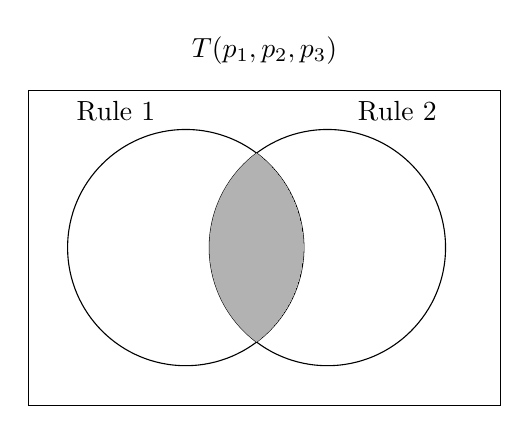
\begin{tikzpicture}
        \draw (-2,-2) -- (4,-2) -- (4,2) -- (-2,2) -- (-2,-2);
        \node at (1,2.5) {$T(p_1, p_2, p_3)$};
        \node [draw, circle, minimum size = 3cm, label={100:Rule 1}] () at (0,0){};
        \node [draw, circle, minimum size = 3cm, label={80:Rule 2}] () at (1.8,0){};
        % Intersection points of circles (needed for next tikzpicture):
        % \fill[red] (0.9, 1.2) circle (1pt);
        % \fill[red] (0.9, -1.2) circle (1pt);
        \begin{scope}
            \clip (0,0) circle (1.5cm);
            \clip (1.8,0) circle (1.5cm);
            \fill[black!30](0,0) circle(1.5cm);
        \end{scope}
        
    \end{tikzpicture}
    \caption{The two sets that should not be considered in the calculation}
    \label{fig:venn_diagram_with_rules}
\end{figure}

The difficulty with this formulation is that the highlighted intersection will
be counted twice and is hard to identify how many such terms there are.
An alternative approach is to break down the Rule 2 subset into three parts as
show in Figure~\ref{fig:venn_diagram_with_subsets}.

\begin{figure}[H]
    \centering
    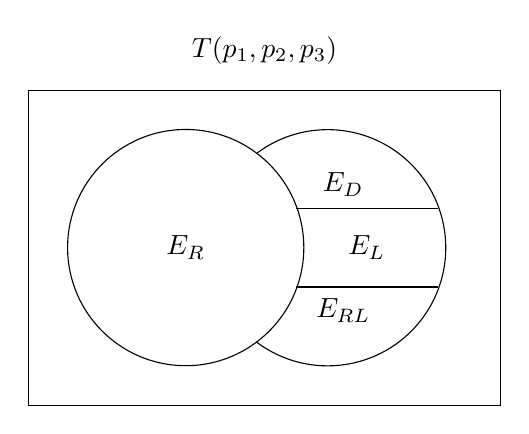
\begin{tikzpicture}
        \draw (-2,-2) -- (4,-2) -- (4,2) -- (-2,2) -- (-2,-2);
        \node at (1,2.5) {$T(p_1, p_2, p_3)$};
        \node [draw, circle, minimum size = 3cm] () at (0,0){};
        \node at (0, 0) {$E_R$};
        \draw (0.9, -1.2) arc (-127:127:1.5cm);
        \node at (2, 0.8) {$E_D$};
        \draw (1.4, 0.5) -- (3.2, 0.5);
        \node at (2.3, 0) {$E_L$};
        \draw (1.4, -0.5) --(3.2, -0.5);
        \node at (2, -0.8) {$E_{RL}$};
    \end{tikzpicture}
    \caption{Splitting rule 1 and rule 2 into multiple subsets without any
    intersections}
    \label{fig:venn_diagram_with_subsets}
\end{figure}

The terms \(E_R, E_L, E_D, E_{RL}\) consist of all cases that should be excluded
based on rule 1 and rule 2.
The term \(E_R(p_1,p_2,p_3)\) denotes the number of permutations that end in
\(R\), which needs to be removed from the total of all permutations so that rule
\ref{rule1} is satisfied.
Having excluded all permutations that end in \(R\), the
permutations that have an \(R\) followed by an \(L\) (rule \ref{rule2}) need to
be excluded as well.
Although, removing all permutations ending in \(R\) was not too complicated,
removing all permutations that follow rule \ref{rule2} is slightly more complex.
This is because equation \(E_R(p_1,p_2,p_3)\) already considers some cases where
there is an \(R\) followed by an \(L\).
Therefore, in order to consider only new cases, permutations of rule~\ref{rule2}
are split into three new terms; \(E_D\), \(E_L\) and \(E_{RL}\).
These terms denote the permutations that have an \(R\) followed by an \(L\) AND
do not end in \(R\).
The term \(E_D\) considers all permutations that end in \(D\) while \(E_L\) the
ones that end in \(L\).
Finally, the last term (\(E_{RL}\)) denotes all permutations that end in \(R\),
\(L\) where there is no other \(R\) followed by an \(L\) in any other position
apart from the last two.
This term is used because in the \(E_L\) term, such cases (where \(R\) and \(L\)
are in the last two positions) are only considered when there is another \(R\)
followed by an \(L\) somewhere.
Thus, the term \(E_{RL}\) is a particular set of permutations that the formula
of \(E_L\) fails to include by itself.

\begin{itemize}
    \item \(T\): All permutations
    \item \(E_R\): Permutations ending with \(R\)
    \item \(E_D\): Permutations ending with \(D\) that have an \(R\) followed by
    an \(L\) somewhere
    \item \(E_L\): Permutations ending with \(L\) that have an \(R\) followed by
    an \(L\) somewhere apart from the end of the array
    \item \(E_{RL}\): Permutations ending in \(R, L\) that do not have an \(R\)
    followed by an \(L\) anywhere else
\end{itemize}


Here's the expression for each of these terms:

\begin{align}
    T(p_1, p_2, p_3) &= \frac{(p_1 + p_2 + p_3)!}{p_1! \times p_2! \times p_3!} \\
    E_R(p_1, p_2, p_3) &= \frac{(p_1 + p_2 + p_3 - 1)!}
    {p_1! \times (p_2-1)! \times p_3!} \\
    E_D(p_1, p_2, p_3) &= \sum_{i=1}^{\min(R,L)} (-1)^{i+1}
    \frac{(p_1 + p_2 + p_3 - i - 1)!}
    {(p_1 - 1)! \times (p_2 - i)! \times (p_3 - i)! \times (i)!} \\
    E_L(p_1, p_2, p_3) &= \sum_{i=1}^{\min(R,L-1)} (-1)^{i+1}
    \frac{(p_1 + p_2 + p_3 - i - 1)!}
    {p_1! \times (p_2 - i)! \times (p_3 - i - 1)! \times (i)!} \\
    E_{RL}(p_1, p_2, p_3) &= \sum_{i=1}^{\min(R,L)} (-1)^{i+1}
    \frac{(p_1 + p_2 + p_3 - i - 1)!}
    {p_1! \times (p_2 - i)! \times (p_3 - i)! \times (i - 1)!}
\end{align}

\begin{align*}
    R(p_1, p_2, p_3) = T(p_1, p_2, p_3) & - E_R(p_1, p_2, p_3) -
    E_D(p_1, p_2, p_3) \\
    & - E_L(p_1, p_2, p_3) - E_{RL}(p_1, p_2, p_3)
\end{align*}

\paragraph{Example of the permutation algorithm}
Consider the term \((\lambda_2) (\lambda_1) \mu^2\) and the above expressions.
In order to get the coefficient of that term the permutation algorithm needs to
be applied with an input of \(p_1=1, p_2=1, p_3=2\), i.e. 1 \(D\), 1 \(R\) and 2
\(L\)s in the array.
The permutations that correspond to each expression can be seen below:

\begin{equation*}
    T(p_1, p_2, p_3) = \frac{(1+1+2)!}{1! \; 1! \; 2!} = 12
\end{equation*}

\begin{align*}
    & [D, R, L, L] \quad [R, D, L, L] \quad [D, L, R, L] \quad
    [R, L, D, L] \quad [D, L, L, R] \quad [R, L, L, D] \\
    & [L, D, R, L] \quad [L, R, D, L] \quad [L, D, L, R] \quad
    [L, R, L, D] \quad [L, L, D, R] \quad [L, L, R, D]
\end{align*}

\begin{equation*}
    E_R(p_1, p_2, p_3) = \frac{(1+1+2-1)!}{1! \; (1-1)! \; 2!} = 3
\end{equation*}

\begin{align*}
    & [D, L, L, | R] \quad [L, D, L, | R] \quad [L, L, D, | R]
\end{align*}


\begin{equation*}
    E_D(p_1, p_2, p_3) = \sum_{i=1}^{1} (-1)^{i+1} \frac{(1+1+2-i-1)!}{0! \;
    (1-i)! \; (2-i)! \; (i)!} = 1 \times \frac{2}{0! \; 0! \; 1! \; 1!} = 2
\end{equation*}

\begin{align*}
    & [R, L, L, | D] \quad [L, R, L, | D]
\end{align*}


\begin{equation*}
    E_L(p_1, p_2, p_3) = \sum_{i=1}^{1} (-1)^{i+1}
    \frac{(1+1+2-i-1)!}{1! \; (1-i)! \; (2-i-1)! \; (i)!}
    = 1 \times \frac{2}{1! \; 0! \; 0! \; 1!} = 2
\end{equation*}

\begin{align*}
    & [D, R, L, | L] \quad [R, L, D, | L]
\end{align*}


\begin{equation*}
    E_{RL}(p_1, p_2, p_3) = \sum_{i=1}^{1} (-1)^{i+1}
    \frac{(1+1+2-i-1)!}{1! \; (1-i)! \; (2-i)! \; (i_1)!}
    = 1 \times \frac{2}{1! \; 0! \; 1! \; 0!} = 2
\end{equation*}

\begin{align*}
    & [D, L, | R, L] \quad [L, D, | R, L]
\end{align*}


Although this method is useful, currently this can be used to find only spanning
trees that are rooted at state \((0,0)\) and for the case of \(C = 1\).
In order to get the steady state probabilities, a more general approach that is
generic to all states \((u,v)\) is needed.
Further work on this specific topic will not be part of this research project.
